%!  pour pdfLatex
\documentclass[a4paper]{article}
%\usepackage[hmargin={1.5cm,1.5cm},vmargin={2.4cm,2.4cm},headheight=13.1pt]{geometry}
\usepackage[a4paper,landscape,twocolumn,
            hmargin=1.8cm,vmargin=2.2cm,headheight=13.1pt]{geometry}

\usepackage[pdftex]{graphicx,color}
\usepackage[pdftex,colorlinks={true},urlcolor={blue},pdfauthor={remy Nicolai}]{hyperref}

\usepackage[T1]{fontenc}
\usepackage[utf8]{inputenc}

\usepackage{lmodern}
\usepackage[frenchb]{babel}

\usepackage{fancyhdr}
\pagestyle{fancy}

\usepackage{floatflt}
\usepackage{maths}

\usepackage{parcolumns}
\setlength{\parindent}{0pt}

\usepackage{caption}
\usepackage{subcaption}

\usepackage{makeidx}

\usepackage[french,ruled,vlined]{algorithm2e}
\SetKwComment{Comment}{\#}{}
\SetKwFor{Tq}{tant que}{}{}
\SetKwFor{Pour}{pour}{}{}
\DontPrintSemicolon
\SetAlgoLined

\usepackage{listings}
\lstset{language=Python,frame=single}
\lstset{literate=
  {á}{{\'a}}1 {é}{{\'e}}1 {í}{{\'i}}1 {ó}{{\'o}}1 {ú}{{\'u}}1
  {Á}{{\'A}}1 {É}{{\'E}}1 {Í}{{\'I}}1 {Ó}{{\'O}}1 {Ú}{{\'U}}1
  {à}{{\`a}}1 {è}{{\`e}}1 {ì}{{\`i}}1 {ò}{{\`o}}1 {ù}{{\`u}}1
  {À}{{\`A}}1 {È}{{\'E}}1 {Ì}{{\`I}}1 {Ò}{{\`O}}1 {Ù}{{\`U}}1
  {ä}{{\"a}}1 {ë}{{\"e}}1 {ï}{{\"i}}1 {ö}{{\"o}}1 {ü}{{\"u}}1
  {Ä}{{\"A}}1 {Ë}{{\"E}}1 {Ï}{{\"I}}1 {Ö}{{\"O}}1 {Ü}{{\"U}}1
  {â}{{\^a}}1 {ê}{{\^e}}1 {î}{{\^i}}1 {ô}{{\^o}}1 {û}{{\^u}}1
  {Â}{{\^A}}1 {Ê}{{\^E}}1 {Î}{{\^I}}1 {Ô}{{\^O}}1 {Û}{{\^U}}1
  {œ}{{\oe}}1 {Œ}{{\OE}}1 {æ}{{\ae}}1 {Æ}{{\AE}}1 {ß}{{\ss}}1
  {ű}{{\H{u}}}1 {Ű}{{\H{U}}}1 {ő}{{\H{o}}}1 {Ő}{{\H{O}}}1
  {ç}{{\c c}}1 {Ç}{{\c C}}1 {ø}{{\o}}1 {å}{{\r a}}1 {Å}{{\r A}}1
  {€}{{\euro}}1 {£}{{\pounds}}1 {«}{{\guillemotleft}}1
  {»}{{\guillemotright}}1 {ñ}{{\~n}}1 {Ñ}{{\~N}}1 {¿}{{?`}}1
}

%pr{\'e}sentation des compteurs de section, ...
\makeatletter
\renewcommand{\thesection}{\Roman{section}.}
\renewcommand{\thesubsection}{\arabic{subsection}.}
\renewcommand{\thesubsubsection}{\arabic{subsubsection}.}
\renewcommand{\labelenumii}{\theenumii.}
\makeatother


\newtheorem*{thm}{Théorème}
\newtheorem{thmn}{Théorème}
\newtheorem*{prop}{Proposition}
\newtheorem{propn}{Proposition}
\newtheorem*{pa}{Présentation axiomatique}
\newtheorem*{propdef}{Proposition - Définition}
\newtheorem*{lem}{Lemme}
\newtheorem{lemn}{Lemme}

\theoremstyle{definition}
\newtheorem*{defi}{Définition}
\newtheorem*{nota}{Notation}
\newtheorem*{exple}{Exemple}
\newtheorem*{exples}{Exemples}


\newenvironment{demo}{\renewcommand{\proofname}{Preuve}\begin{proof}}{\end{proof}}
%\renewcommand{\proofname}{Preuve} doit etre après le begin{document} pour fonctionner

\theoremstyle{remark}
\newtheorem*{rem}{Remarque}
\newtheorem*{rems}{Remarques}

%\usepackage{maths}
%\newcommand{\dbf}{\leftrightarrows}

%En tete et pied de page
\lhead{Informatique}
%\chead{Introduction aux systèmes informatiques}
\rhead{MPSI B Hoche}
\lfoot{\tiny{Cette création est mise à disposition selon le Contrat\\ Paternité-Partage des Conditions Initiales à l'Identique 2.0 France\\ disponible en ligne http://creativecommons.org/licenses/by-sa/2.0/fr/  
} 
\rfoot{\tiny{Rémy Nicolai \jobname \; \today } }
}
\makeindex

\usepackage{parcolumns}
\setlength{\parindent}{0pt}
\makeindex

\begin{document}
\lhead{cours IPT}
\chead{cours 1: Introduction à l'utilisation de Python le 11 09 2019}


\section{Langage de programmation}
Un \emph{langage de programmation} \index{langage de programmation} est un ensemble fixé de mots (appelés mots \og réservés\fg) et d'un ensemble de règles (la syntaxe)\index{syntaxe}. Un texte constitué de mots réservés \index{mot réservé} ou non peut être qualifié de \emph{code} \index{code} lorsqu'il respecte les règles.\newline
La \emph{syntaxe} est l'ensemble de règles que doit vérifier un texte pour pouvoir être qualifié de \og code\fg valide pour le langage. Dans le contexte de la programmation, un code est simplement un texte vérifiant ces règles et \og coder\fg signifie simplement écrire du code. Autrement dit, un code est un texte \og correct\fg pour la syntaxe.\newline
Les codes sont des énoncés \emph{performatifs} \index{énoncé permormatif} c'est à dire dont le but est de faire (ou plutôt de faire faire) quelque chose. 
Un code peut être traduit par un programme (spécifique au langage) en une succession d'ordres donnés à une machine. Cette succession d'actions doit exécuter la tâche pour laquelle le code a été écrit. Cela peut se faire en une fois (\emph{langage interprété}) ou en deux fois (\emph{langage compilé}). \index{langage interprété} \index{langage compilé}\newline
Pour un langage interprété, le \og traducteur\fg est appelé \emph{interpréteur} \index{interpréteur}. L'appel de l'interpréteur avec un code donné en paramètre exécute directement la tâche. Python, qui est le langage utilisé en mpsi, est un langage interprété.\newline
Pour un langage compilé, le \og traducteur\fg est appelé \emph{compilateur}. \index{compilateur} L'appel du compilateur avec un code donné en paramètre produit un autre programme. Dans un second temps, l'appel de ce programme réalise la tâche visée.\newline

\section{Environnement de programmation}
Un \emph{environnement de programmation} \index{environnement de programmation} est une collection de dispositifs permettant de coder et d'exécuter du code.
\subsection{Interpréteur utilisé interactivement}
Le plus simple des environnements est l'interpréteur lui même utilisé interactivement. Il suffit de l'appeler (le nom peut varier selon les systèmes : \texttt{python} ou \texttt{python3} par exemple) sans paramètre dans une \emph{console}. Une console est une application dont l'interface avec l'utilisateur est uniquement du texte (ligne de commandes)\index{console}. On trouve aussi le mot \emph{terminal} pour désigner une console.\newline
L'interpréteur attend une ligne de code (correcte) et l'exécute directement après \texttt{entrée}. Cet environnement est commode pour une initiation ou de petites vérifications. 
On peut dire que l'interpréteur Python est lui même une console qui attend des commandes correctes.
Il a deux limitations immédiates: la difficulté d'exécuter un code contenant plusieurs lignes, le fait que le code exécuté n'est pas enregistré en tant que fichier et donc difficile à réutiliser.

\subsection{Couple éditeur-console}
Un environnement de programmation très simple est constitué par un couple éditeur-console.\newline
L'éditeur\footnote{à ne pas confondre avec un traitement de texte} de texte \index{éditeur de texte} \index{traitement de texte} permet de coder et d'enregistrer le code dans un fichier (l'extension du nom de fichier est .py \index{extension de nom de fichier}).\newline
Pour exécuter le code, dans une console, on appelle l'interpréteur en lui donnant le nom du fichier de code en paramètre.\newline
Sous diverses réserves (en particulier sous Windows des problèmes de \emph{chemins de dossier} peuvent se produire), cela peut se faire dans n'importe quelle console. Sous windows un éditeur simple est notepad. En général, un éditeur propose une \emph{coloration syntaxique} \index{coloration syntaxique} spécifique à Python. Il est conseillé de l'activer.

\subsection{Autres environnements: spyder}
Il existe de nombreux environnements de programmation pour Python offrant bien d'autres ressources (inspection des variables, debogage, ...) Un environnement de programmation sophistiqué est très utile au programmeur expérienté mais plutôt nuisible au débutant car l'apprentissage de l'environnement vient s'ajouter à celui du langage proprement dit.\newline
Toutefois le programme officiel de la classe nous demande d'utiliser Python par l'intermédiaire de l'environnement de programmation spyder. Les machines des salles de TP du lycée sont équipées de Spyder. Il est conseillé de l'installer sur vos machines personnelles de manière à ne pas être désorienté si vous devez l'utiliser en concours. 

Un environnement de travail est constitué de plusieurs fenêtres (Figure \ref{fig:spyder}) qui doivent permettre les deux modes d'utilisation. Les environnements évolués comme Spyder offrent d'autres fonctionalités\footnote{par exemple des outils de vérification (débogage).}.
\begin{itemize}
 \item Dans une fenêtre console/interpréteur, on peut écrire directement une intruction Python et l'exécuter en tapant "Entrée". 
 \item Dans la fenêtre "Editeur de texte" on peut écrire, enregistrer, ... des fichiers d'extension \verb|.py| puis les faire exécuter (bouton Executer du menu ou flèche verte (suivant les versions)) dans une fenêtre console/interpréteur)
\end{itemize}
 
 \begin{figure}[h!]
 \centering
 %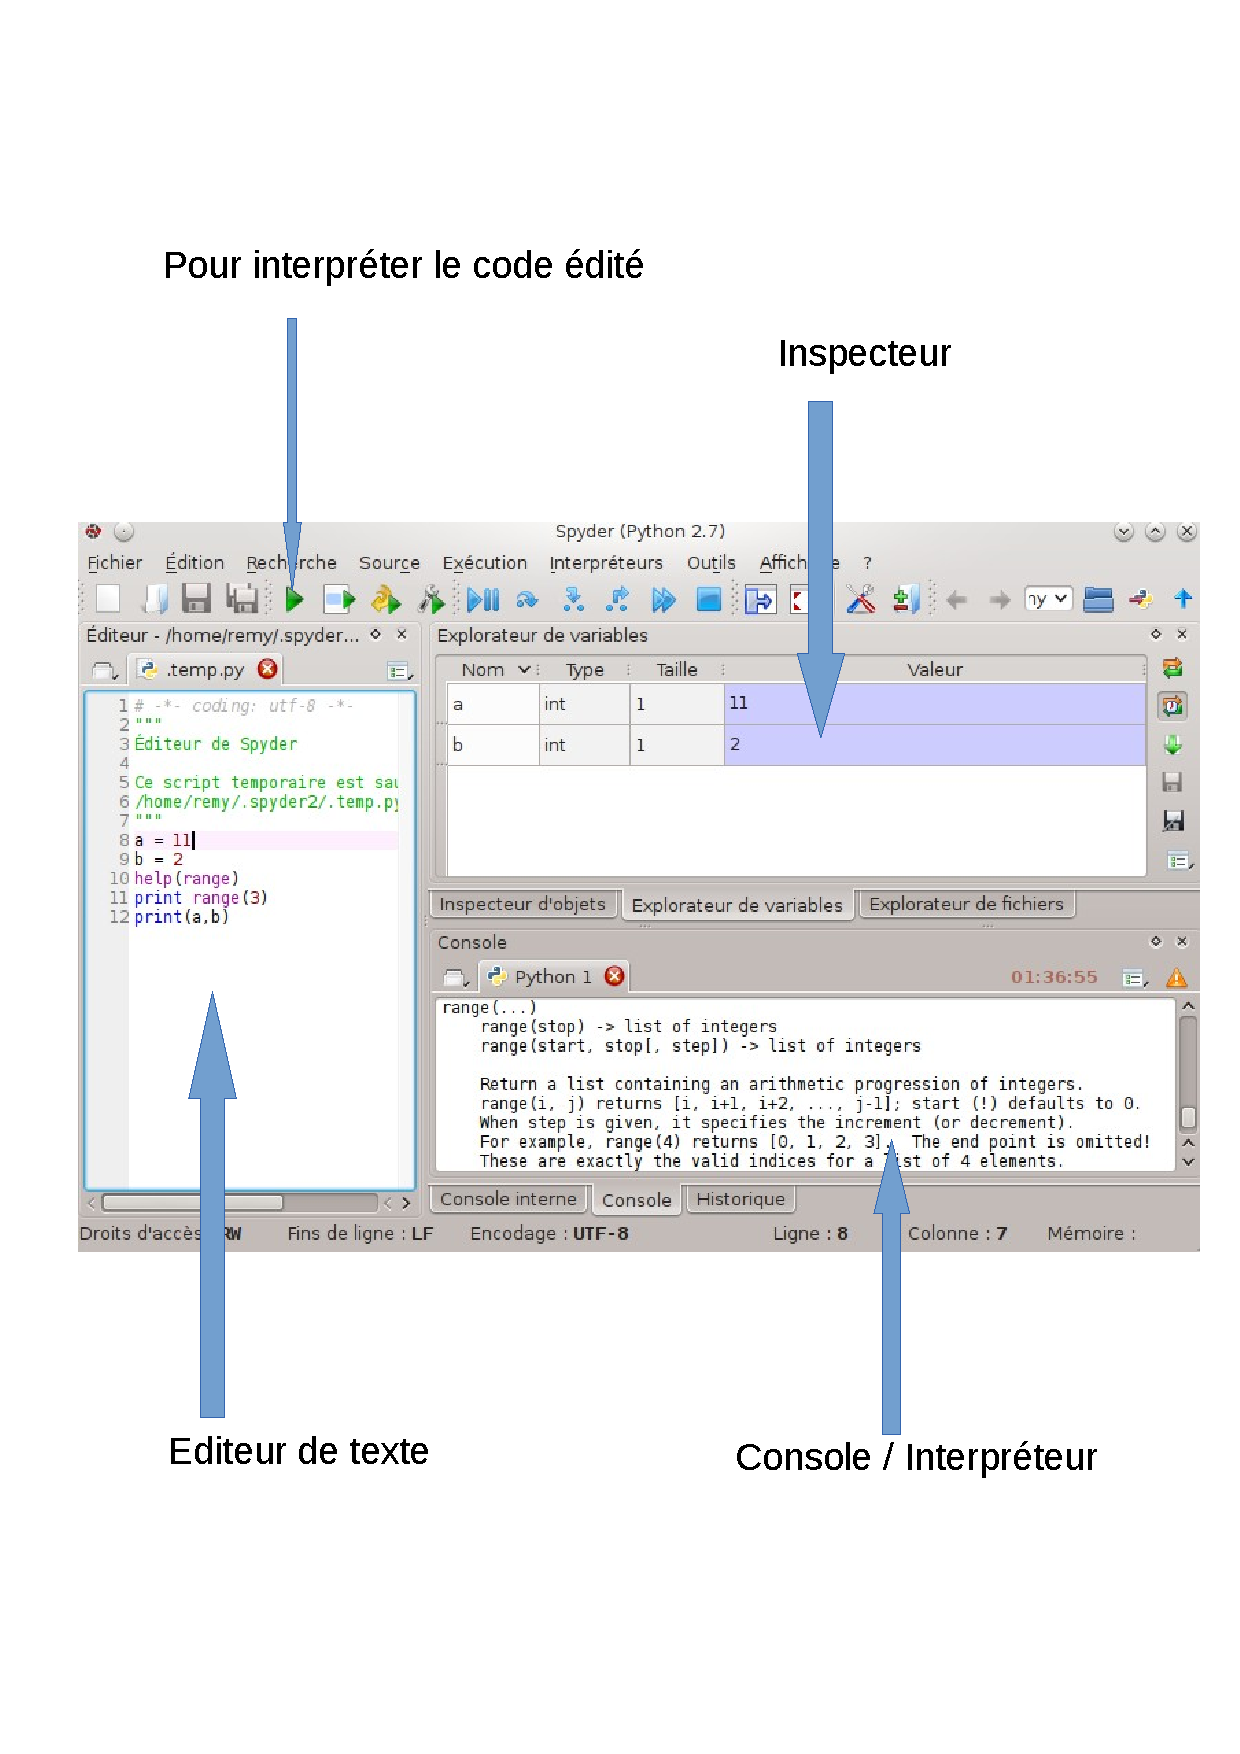
\includegraphics[width=10cm,keepaspectratio=true]{./spyder.pdf}
 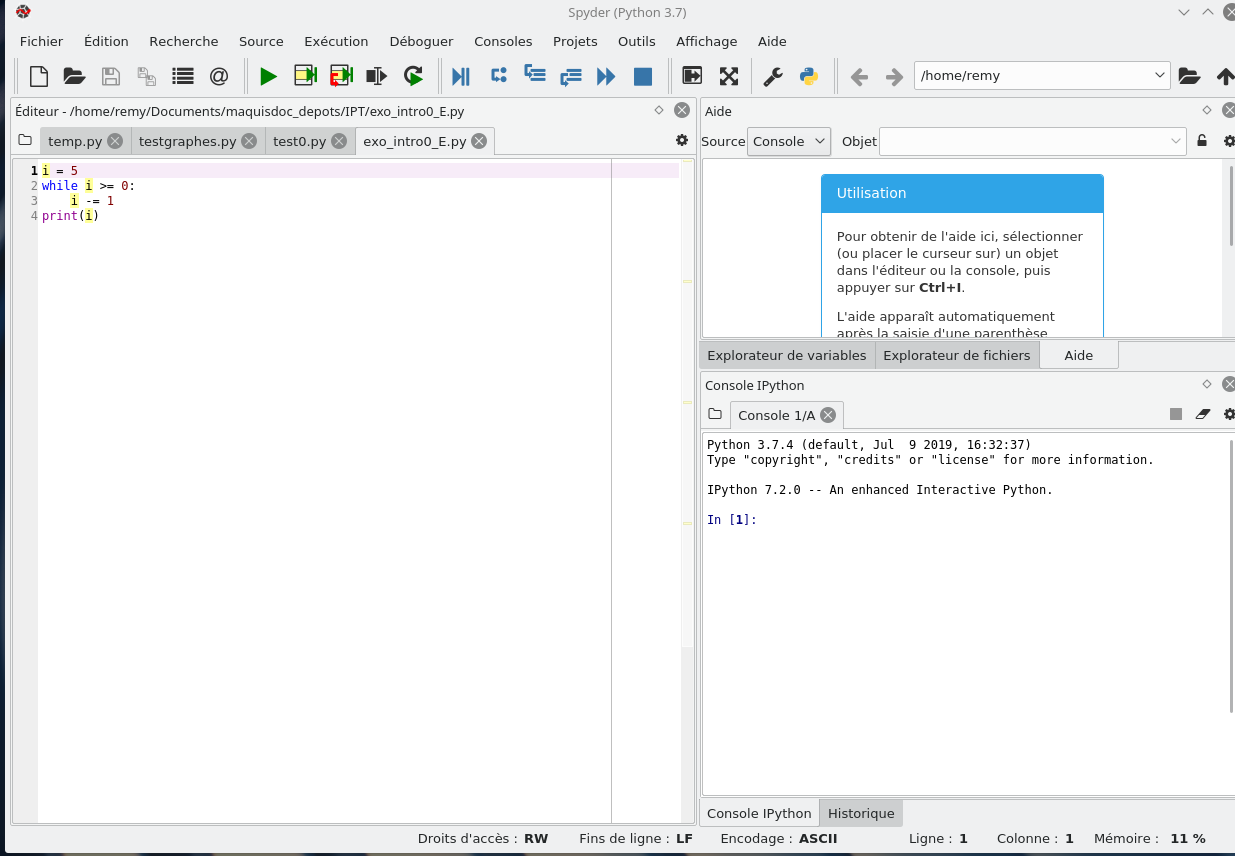
\includegraphics[width=10cm]{environnement_1.png}
 % spyder.pdf: 595x842 pixel, 72dpi, 20.99x29.70 cm, bb=0 0 595 842
 \caption{Environnement de développement spyder}
 \label{fig:spyder}
\end{figure}


Exemple avec les instructions \texttt{1+1} et \texttt{print "coucou"} ou \texttt{print("coucou")} à interpréter directement ou à exécuter par l'intermédiaire d'un fichier. Lors de l'utilisation d'un fichier, bien maitriser sa place dans l'arborescence des disques.

Il arrive souvent que le code soit mal écrit et conduise à un processus qui ne s'arrête jamais (boucle infinie). Il faut savoir comment l'arrêter.
Par exemple
 \begin{verbatim}
i = 0
while 0 < 10:
    print('coucou'+str(i))
    i+=1
 \end{verbatim}
\emph{Bien respecter l'indentation} c'est à dire les espaces en début de ligne. Faites interpréter ce code avec avec la flèche verte (dans Spyder). Comme on a formé délibérément une \emph{boucle infinie} \index{boucle infinie}, il faut pouvoir forcer l'arrêt de l'interpréteur. La fenêtre de l'interpréteur contient en principe un bouton permettant de le faire. En général ce bouton est placé en haut à droite de la ligne de menu. Sa forme dépend de l'environnement: petit triangle jaune avec un point d'exclamation, carré rouge, ....
On peut citer d'autres environnements, notamment des interpréteurs en ligne: par exemple \href{http://shell.appspot.com}{shell.appspot.com} ou \href{http://live.sympy.org/shellmobile}{live.sympy.org/shellmobile} qui est adapté aux écrans de smartphone et orienté calcul formel  (utilisant le module sympy). 

%\clearpage

\section{Exemples d'instructions}
Diverses instructions sont proposées dans la colonne de gauche. On se propose de les faire interpréter et de comprendre ce qui est renvoyé à l'aide des commentaires fournis dans la colonne de droite.
\begin{parcolumns}[rulebetween,distance=1cm,colwidths={1= .35\linewidth}]{2}
  \colchunk{\texttt{128, id(128), type(128)}}
  \colchunk{\texttt{128} est l'expression littérale \index{littéral} du nombre $128$ et \texttt{id(128)} renvoie l'identifiant unique de cet objet dans la mémoire de l'interpréteur, \texttt{type(128)} renvoie son type.}
  \colplacechunks
  
  \colchunk{
  \begin{verbatim}
   5 ** 5
   5 ** 200
  \end{verbatim}
  }
  \colchunk{Les entiers ne sont pas limités. En Python 2.7, le "L" à la fin signifie que le résultat est un entier "long" c'est à dire trop grand pour être représenté par un mot machine. Python sait gérer ces entiers; en cas d'opération dans laquelle intervient un entier long, le résultat est toujours un entier long. En Python 3, on peut dire pour simplifier que tous les entiers sont longs et le marqueur "L" n'est plus utilisé}
  \colplacechunks
  
  \colchunk{
  \begin{verbatim}
   14 // 3
   14 % 3
   14.1 / 3.0
  \end{verbatim}
  }
  \colchunk{Dans une division euclidienne, le quotient est obtenu par //, le reste par \%.\newline
  En Python 2 le / entre deux entiers calcule le quotient entier de la division euclidienne alors qu'en Python 3 il calcule une valeur approchée (float: nombres en virgule flottante) du quotient rationnel.\newline
  Bonne pratique: réserver le / à une division entre nombres en virgule flottante. Bien noter que les opérations entre entiers en virgule flottante sont toujours approchées.}
  \colplacechunks
  
  \colchunk{
  \begin{verbatim}
   pi
   sin(pi)
  \end{verbatim}
  }
  \colchunk{Python n'est pas spécialement orienté vers les maths. $\pi$ n'est pas un décimal, $\sin$ est inconnu.}
  \colplacechunks
\end{parcolumns}

\begin{parcolumns}[rulebetween,distance=1cm,colwidths={1= .35\linewidth}]{2}
  \colchunk{
  \begin{verbatim}
   from math import sin
   sin(pi)
   cos(3.1)
   from math import *
   cos(3.1)
  \end{verbatim}
  }
  \colchunk{Si on veut utiliser des opérations mathématiques, on doit les importer de la bibliothèque mathématique. Le "*" permet de tout importer ce qui n'est pas une bonne pratique. Il vaut mieux garder l'espace de nommage aussi petit que possible. Noter que le nom du module est \texttt{math} sans \og s\fg.}
  \colplacechunks
  
  \colchunk{
  \begin{verbatim}
   type(42)
   type(4.2)
   type(5 ** 20)
  \end{verbatim}
  }
  \colchunk{Les entiers et les nombres en virgule flottante sont des types élémentaires de valeurs pour le langage Python}
  \colplacechunks
  
  \colchunk{
  \begin{verbatim}
    i = 1.0j
    c = i ** 2
    i, c
    type(i), type(c)
  \end{verbatim}
  }
  \colchunk{Python connait les nombres complexes. La première ligne contient une expression littérale complexe.
  }
  \colplacechunks
 
  \colchunk{
  \begin{verbatim}
   help(floor)
   int(3.2)
   int(-3.2)
   help(int)
   int("abc",16)
  \end{verbatim}
  }
  \colchunk{On peut trouver de l'aide sur une fonction dont on connait le nom en utilisant la fonction \verb|help|. Que font les fonctions \verb|ceil| ou \verb|round| ? Que renvoie la fonction \verb|int|? Les valeurs renvoyées par \verb|int(3.5)| et \verb|round(3.5)| sont-elles les mêmes pour Python?}
  \colplacechunks
\end{parcolumns}

Pour insérer un \emph{commentaire} c'est à dire une ligne qui est ignorée par l'interpréteur et ne sert qu'à aider le programmeur, il suffit de la faire commencer par un dièse \#. Pour insérer des commentaires sur plusieurs lignes, il faut les encadrer par deux lignes contenant seulement  """.



\section{Concepts et premiers éléments de syntaxe}
L'objet de ce document est d'introduire ces premiers éléments de syntaxe ainsi que du vocabulaire et des concepts permettant de les comprendre. Ce cours est très limité et il est indispensable de savoir chercher dans la \href{http://docs.python.org/3.3/reference/}{documentation officielle} des informations plus précises. Sans une certaine maitrise du vocabulaire et des concepts, naviguer dans la documentation est très difficile.
\subsection{Expressions}
Une expression\index{expression} est une phrase que l'interpréteur peut évaluer à un objet. La liste suivante présente les principaux types d'éléments constituants une expression.
\begin{description}
 \item[nom] ou variable\index{nom} : des mots formés avec les lettres de a à z en minuscule ou majuscule (Python est sensible à la casse c'est à dire que \verb|Cassy| et \verb|cassy| sont deux noms différents), le caractère underscore \verb|_| et les chiffres de \verb|0| à \verb|9| (sauf pour le premier caractère). Si un mot est réservé par Python pour un usage prédéfini, il ne peut pas être un nom.
 \item[littéral] : \index{litteral} un littéral désigne un objet fixé et pré-défini. La syntaxe dépend du type d'objet représenté, retenir seulement les cas suivants.\newline
Les délimiteurs "espace" pour les entiers (int) avec éventuellement \verb|-|: par exemple \verb| 12 | désigne le nombre $12$. Il faut seulement le séparer d'un autre mot par des espaces.\newline
Les délimiteurs \verb|" "| ou \verb|' '| pour les chaînes de caractères: \verb|"coucou"| est une chaîne de caractères.\newline
Le \verb|.| pour les objets du type float: \verb|1.1| est un objet du type float, \verb|1.0| est un objet du type float alors que \verb|1| est un objet du type int et que \verb|"1"| est un objet du type str (chaîne de caractère).\newline
Le \verb|j| pour un type "complex" : \verb|1.0j| représente l'imaginaire pur $i$. Noter que la partie imaginaire est de type float. Pour former des complexes avec une partie réelle non nulle, utiliser \verb|+| et un littéral du type float.

\item[opérateurs] \index{opérateur} Un opérateur est un mot (contenant en général seulement un ou deux caractères) placé entre deux expressions (les opérandes). La phrase ainsi formée est elle même une expression. Il existe une hiérarchie entre les opérateurs qui élimine les ambiguités lorsque plus de deux opérateurs interviennent. Les parenthèses \verb|()| sont utilisées lorsque cette hierarchie n'est pas très claire. Pour qu'une telle phrase soit correcte, les opérandes doivent représenter des objets dont le type est en accord avec l'opérateur. Le résultat de l'évaluation est un objet dont le type dépend de l'opérateur.  
\end{description}
Présentons les opérateurs à retenir en les classant suivant le type de l'objet produit par l'évaluation de l'expression.
\begin{description}
 \item[opérateurs arithmétiques] Le résultat est d'un type représentant un nombre (en convenant que num designe l'un ou l'autre des types \verb|int| ou \verb|float|). Pour les opérateurs présentés dans le tableau suivant, il est conseillé de se limiter à des expressions dans les lesquelles les opérandes sont de type indiqué, le résultat de l'opération est alors de même type.
 {%
\begin{center}
\begin{tabular}{cccccc}
addition & multiplication & puissance & reste & quotient & division \\
\verb|+| & \verb|*| & \verb|**| & \verb|%| & \verb|//|& \verb|/|    \\
num      & num      & num       & int      & int      & float    \\
 \end{tabular}
 \end{center}
}%

\item[opérateurs booléens] Les opérandes sont de type booléens, l'expression formée s'évalue en booléen. 
\begin{center}
\begin{tabular}{ccc}
\verb|and| & \verb|or| & \verb|not| \\
 \end{tabular}
\end{center}
On peut remarquer que \verb|not| n'est pas tout à fait à sa place car il s'agit d'un opérateur \emph{unaire} qui se place à gauche d'une expression booléenne.

\item[opérateurs sur les chaînes de caractères] Le seul à retenir pour le moment est l'opérateur de \emph{concaténation} \index{concaténation} qui se note \verb|+|.\newline
Il colle bout à bout deux chaînes :
\begin{verbatim}
 "tagada"+"tsoin tsoin"
\end{verbatim}
s'évalue à \verb|"tagadatsoin tsoin"|.

\item[opérateurs de comparaison] Une condition est une expression qui s'évalue en une valeur booléenne. Les opérateurs de comparaison forment des conditions. Les caractères utilisés pour les opérateurs présentés dans le tableau suivant sont assez clairs quant à leur signification. 
{%
\begin{center}
\begin{tabular}{cccccc}
\verb|==|  & \verb|!=| & \verb|>|  & \verb|<|  & \verb|>=|  &  \verb|<=|
 \end{tabular}
 \end{center}
}
sauf peut être \verb|!=| qui signifie \og est différent de\fg. Le détail de ce que fait l'opérateur == mériterait d'être approfondi suivant les types des objets comparés.

\item[opérateurs d'affectation] Ils sont de nature très différentes des précédents. Ce qui est à gauche d'un tel opérateur doit être un nom, ce qui est à droite est une expression. L'exécution référence par le nom à gauche un objet évalué à partir de l'expression de droite.\newline
Le principal opérateur de ce type est \verb|=| que l'on peut appeler assignation simple. Le nom à gauche référence l'objet évalué à droite.\newline
Il existe aussi des \emph{assignations augmentées} par des opérateurs
\begin{center}
\begin{tabular}{cccccc}
\verb|+=|  & \verb|*=| & \verb|/=|  & \verb|%=|
 \end{tabular}
 \end{center}
Par exemple \verb|a += 1| revient exactement au même que \verb|a = a + 1|. Les autres opérateurs sont sur le même principe.
\end{description}
Le mélange de divers types d'objets dans des expressions soulève de délicates questions qui méritent un examen détaillé de la documentation officielle du langage. Il vaut mieux le remttre à plus tard quand vous aurez plus d'expérience\newline
Une particularité de Python est qu'il permet des assignations multiples.\newline
Après \verb|a , b = c , d|, les noms \verb|a| et \verb|c| désignent le même objet (celui que désignait \verb|c| avant l'exécution) et de même pour \verb|b| et \verb|d|. Cela permet en particulier de permuter les noms de deux objets.\newline
Supposons que \verb|a| désigne l'objet1 et \verb|b| désigne l'objet2, et exécutons \verb|a , b = b , a|. Les noms sont alors permutés : \verb|a| désigne l'objet2 et \verb|b| désigne l'objet1 sans que les objets soient modifiés.

\subsection{Instructions}
Du point de vue de la syntaxe, une instruction\footnote{Le terme utilisé pour \og instruction\fg en anglais est \emph{statement}.} est une \emph{ligne de code}.\newline
L'\emph{indentation}, c'est à dire les caractères \og espaces\fg~ présents au début d'une ligne joue un rôle très important dans la syntaxe Python.\newline
Certaines constructions peuvent se poursuivre sur plusieurs lignes. Il existe aussi des moyens de faire continuer le texte d'une instruction sur plusieurs lignes en utilisant des caractères spéciaux voir la documentation sur "logical line", "physical line", "line joining".\newline
Un bloc d'instructions est une séquence d'intructions qui se suivent.
\subsubsection{Commentaires}
Un commentaire est un texte qui n'est pas interprété par Python. Lorsque l'interpréteur rencontre le caractère \verb|#|, il ignore le texte qui le suit jusqu'à la fin de la ligne. Pour insérer une ligne de commentaire, il suffit donc de la faire commencer par \verb|#|.\newline
Si on veut insérer un commentaire sur plusieurs lignes sans les faire débuter par dièse, on peut utiliser 
\begin{verbatim}
 """
ligne 1 de commentaire
ligne 2
...
"""
\end{verbatim}
sauf dans certaines circonstances, le texte entre les délimiteurs \verb|"""| sera ignoré par l'interpréteur. Ceci n'est toutefois pas un véritable commentaire (voir la documentation). 

\subsubsection{Instructions conditionnelles}
Une instruction conditionnelle ou un bloc conditionnel d'instructions \index{bloc conditionnel} ne s'exécute que si une certaine condition est évaluée à vrai. La syntaxe est de la forme suivante
\begin{verbatim}
if condition :
  instruction1
  instruction2
  ...
  instructionN
instructiontoujoursinterpretee
\end{verbatim}
Noter le \verb|:| dans la première ligne et l'indentation qui \emph{délimitent} le bloc d'instructions. Utilisez quatre espaces (pas de tabulation) pour l'indentation.\newline
Il existe des variantes avec des \verb|else :| ou des \verb| elif condition1 :| qui ne sont pas présentées ici mais qui seront abordées en TP.

\subsubsection{Boucles conditionnelles}
Une boucle conditionnelle est un bloc d'instructions \index{boucle conditionnelle} qui sera exécuté tout entier tant qu'une certaine condition est évaluée à vrai. La syntaxe est la suivante
\begin{verbatim}
instructiondavant
while condition :
  instruction1
  instruction2
  ...
  instructionN
instructiondapres
\end{verbatim}
Bien noter que le bloc peut n'être jamais exécuté car l'évaluation de la condition se fait avant la première exécution. Il est aussi possible que se produise une \emph{boucle infinie} lorsque les exécutions du blocs ne changent pas l'évaluation de la condition.\newline
La syntaxe des boucles inconditionnelles utilisant le mot réservé \og for\fg n'est pas présentée ici. En Python, leur nature est complètement différente et intimement reliées à certains types particuliers d'objets.

\section{Objets, Noms, Assignations}
\subsection{Principes}
En Python\footnote{ce paragraphe est tiré de du paragraphe "Data model" de la documentation officielle du projet Python.} le concept d'\emph{objet} englobe tous les types de données. 
Chaque objet a un \emph{identifiant}, un \emph{type} et une \emph{valeur}.\newline
Une fois qu'un objet est créé, son identifiant ne change jamais; on peut le voir comme \emph{l'adresse} de l'objet dans la mémoire.\footnote{L'\emph{opérateur} \texttt{is} compare les identifiants de deux objets, la \emph{fonction} \texttt{id()} renvoie un nombre représentant son identité.}\newline
Le type d'un objet est aussi fixé une fois que l'objet est créé.\footnote{On peut dire qu'un objet est une \emph{instance} de son type. Une création (construction) est une instanciation de type (classe).} Ce type détermine les opérations que l'objet supporte (ex.: a-t-il une longueur?) et les valeurs qu'il peut prendre. Les types d'objets Python comprennent en particulier diverses sortes de nombres, chaîne de caractères, \emph{tuple}, liste, dictionnaire.\newline
Suivant son type, un objet peut être \emph{modifiable} ou \emph{non-modifiable}\footnote{mutable immutable}. Cela correspond bien au sens courant du mot objet: un objet du type \texttt{thermos} est modifiable, le même objet peut contenir plus ou moins de café. En revanche l'objet \texttt{nombre entier 2} ~n'est pas modifiable. En Python les types numériques ou le type chaîne de caractère ne sont pas modifiables alors que le type liste est modifiable.\newline
Les objets ne sont jamais explicitement détruits\footnote{contrairement à d'autres langage par exemple \texttt{C}.}; dès qu'il devient impossible de les atteindre, un dispositif de \emph{ramasse-miettes}\footnote{garbage collector} se charge de le détruire pour libérer des ressources.\newline
L'accès à un objet ne se fait pas à l'aide de son identifiant mais à partir d'un \emph{nom}. L'opération de nommage qui consiste essentiellement à écrire quelque part sur un registre une association entre un nom et un identifiant (analogue en cela au passage en mairie pour une déclaration de naissance) s'appelle une \emph{assignation}.\newline 
La \emph{syntaxe} d'une assignation est de la forme suivante:
\begin{verbatim}
  nono = 1+1
\end{verbatim}
ce qui est à gauche de l'égalité est un \emph{nom}, ce qui est à droite est une \emph{expression}. L'exécution d'une telle instruction revient à
\begin{itemize}
  \item évaluer l'expression de droite à un certain objet
  \item écrire quelque part dans un registre que le nom à gauche désigne cet objet.
\end{itemize}
Le même objet peut très bien avoir plusieurs noms lorsqu'il est le résultat de l'évaluation à droite de plusieurs assignations (on parle alors d'\emph{alias} pour cet objet). En revanche un nom désigne un seul objet. Si un nom est réassigné à un nouvel objet, il est possible que l'objet qu'il désignait avant la réassignation n'ait plus de nom et soit donc inaccessible. Le travail du ramasse miette consiste à examiner le registre pour savoir si c'est le cas et éventuellement libérer de la mémoire.\newline 
En programation Python, la terminologie \og assignation\fg et \og nom\fg est préférable à \og égalité\fg et \og variable\fg.

\subsection{\'Echange de noms}
Dans certains langages, ce qui est à gauche d'un signe \texttt{=} doit être vu comme une sorte de récipient et l'assignation comme le dépôt d'une valeur dans ce récipient. Cette image n'est pas satisfaisante en Python et le but de cette section est de faire comprendre que l'interprétation comme un nommage est meilleure.

\begin{figure}[!ht]
 \centering
 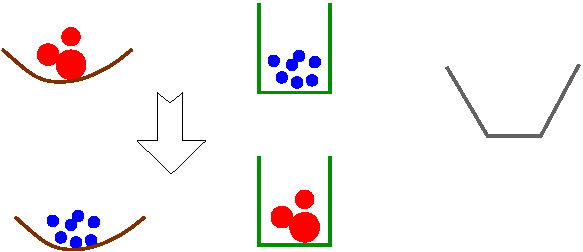
\includegraphics{Einterv_1.pdf}
 \caption{Intervertir les contenus de deux récipients}
 \label{fig:Einterv_1}
\end{figure}

Imaginons que l'on dispose de deux récipients contenant des objets. On veut les échanger. On sent bien qu'un troisième récipient est nécessaire et qu'il est alors facile de l'utiliser transitoirement.(Figure \ref{fig:Einterv_1})\newline
Dans la vraie vie, un récipient se \emph{vide} dans un autre ce qui n'est pas le cas avec des noms et des assignations. On pourrait imaginer que le récipient ne se vide pas mais que son contenu se duplique, ce n'est pas le cas non plus.

Considérons le code Python suivant
\begin{verbatim}
# initialisation
nom1 = "MickeydeTravers"
nom2 = "PetitsRondsBleus"
#Echange
nom3 = nom1
nom1 = nom2
nom2 = nom3
#Verification
print(nom1)
print(nom2)
\end{verbatim}
Après l'exécution de la première ligne du code ci dessus, quel est le type de l'objet désigné par \texttt{nom1}?
Quelle commande supplémentaire peut-on faire exécuter pour s'assurer qu'une assignation "ne vide pas" le nom placée à droite ?
Expliquez pourquoi le code suivant prouve que l'assignation ne copie pas les valeurs.
\begin{verbatim}
# initialisation
nom1 = ["disqueRouge1","disqueRouge2","disqueRouge3"]
nom2 = "PetitsRondsBleus"
print("valeurs initiales")
print(nom1)
print(nom2)

#Echange
nom3 = nom1
nom1 = nom2
nom2 = nom3

#Verification
print("échange")
print(nom1)
print(nom2)

print("modification")
print(nom3)
nom3.remove("disqueRouge2")
print(nom3)
print(nom2)
\end{verbatim}
Après l'exécution de la première ligne du code ci dessus, l'objet désigné par \texttt{nom1} est d'un type cité dans la partie 1. Principes; quel est ce type? Une propriété de ce type explique les résultats de l'exécution de ce code; laquelle? \newline
En utilisant une terminologie venant d'autres langages, on peut dire que l'assignation en Python se fait toujours \emph{par référence} et non \emph{par valeur}. C'est la raison fondamentale pour laquelle l'utilisation du mot \emph{nom} est préférable à celle de \emph{variable}.


\printindex
\end{document}
